\documentclass{beamer}
\usepackage{amsmath}
\usepackage[english]{babel} %set language; note: after changing this, you need to delete all auxiliary files to recompile
\usepackage[utf8]{inputenc} %define file encoding; latin1 is the other often used option
\usepackage{csquotes} % provides context sensitive quotation facilities
\usepackage{graphicx} %allows for inserting figures
\usepackage{booktabs} % for table formatting without vertical lines
\usepackage{textcomp} % allow for example using the Euro sign with \texteuro
\usepackage{stackengine}
\usepackage{wasysym}
\usepackage{tikzsymbols}
\usepackage{textcomp}
\usepackage{xcolor}
\usepackage[dvipsnames]{xcolor}
\usepackage{colortbl}
\usepackage{adjustbox}
\usetikzlibrary{decorations.pathreplacing}
\newcommand{\bubblethis}[2]{
        \tikz[remember picture,baseline]{\node[anchor=base,inner sep=0,outer sep=0]%
        (#1) {\underline{#1}};\node[overlay,cloud callout,callout relative pointer={(0.2cm,-0.7cm)},%
        aspect=2.5,fill=yellow!90] at ($(#1.north)+(-0.5cm,1.6cm)$) {#2};}%
    }%
\tikzset{face/.style={shape=circle,minimum size=4ex,shading=radial,outer sep=0pt,
        inner color=white!50!yellow,outer color= yellow!70!orange}}
%% Some commands to make the code easier
\newcommand{\emoticon}[1][]{%
  \node[face,#1] (emoticon) {};
  %% The eyes are fixed.
  \draw[fill=white] (-1ex,0ex) ..controls (-0.5ex,0.2ex)and(0.5ex,0.2ex)..
        (1ex,0.0ex) ..controls ( 1.5ex,1.5ex)and( 0.2ex,1.7ex)..
        (0ex,0.4ex) ..controls (-0.2ex,1.7ex)and(-1.5ex,1.5ex)..
        (-1ex,0ex)--cycle;}
\newcommand{\pupils}{
  %% standard pupils
  \fill[shift={(0.5ex,0.5ex)},rotate=80] 
       (0,0) ellipse (0.3ex and 0.15ex);
  \fill[shift={(-0.5ex,0.5ex)},rotate=100] 
       (0,0) ellipse (0.3ex and 0.15ex);}

\newcommand{\emoticonname}[1]{
  \node[below=1ex of emoticon,font=\footnotesize,
        minimum width=4cm]{#1};}
\usepackage{scalerel}
\usetikzlibrary{positioning}
\usepackage{xcolor,amssymb}
\newcommand\dangersignb[1][2ex]{%
  \scaleto{\stackengine{0.3pt}{\scalebox{1.1}[.9]{%
  \color{red}$\blacktriangle$}}{\tiny\bfseries !}{O}{c}{F}{F}{L}}{#1}%
}
\newcommand\dangersignw[1][2ex]{%
  \scaleto{\stackengine{0.3pt}{\scalebox{1.1}[.9]{%
  \color{red}$\blacktriangle$}}{\color{white}\tiny\bfseries !}{O}{c}{F}{F}{L}}{#1}%
}
\usepackage{fontawesome} % Social Icons
\usepackage{epstopdf} % allow embedding eps-figures
\usepackage{tikz} % allows drawing figures
\usepackage{amsmath,amssymb,amsthm} %advanced math facilities
\usepackage{lmodern} %uses font that support italic and bold at the same time
\usepackage{hyperref}
\usepackage{tikz}
\hypersetup{
    colorlinks=true,
    linkcolor=blue,
    filecolor=magenta,      
    urlcolor=blue,
}
\usepackage{tcolorbox}
%add citation management using BibLaTeX
\usepackage[citestyle=authoryear-comp, %define style for citations
    bibstyle=authoryear-comp, %define style for bibliography
    maxbibnames=10, %maximum number of authors displayed in bibliography
    minbibnames=1, %minimum number of authors displayed in bibliography
    maxcitenames=3, %maximum number of authors displayed in citations before using et al.
    minnames=1, %maximum number of authors displayed in citations before using et al.
    datezeros=false, % do not print dates with leading zeros
    date=long, %use long formats for dates
    isbn=false,% show no ISBNs in bibliography (applies only if not a mandatory field)
    url=false,% show no urls in bibliography (applies only if not a mandatory field)
    doi=false, % show no dois in bibliography (applies only if not a mandatory field)
    eprint=false, %show no eprint-field in bibliography (applies only if not a mandatory field)
    backend=biber %use biber as the backend; backend=bibtex is less powerful, but easier to install
    ]{biblatex}
\addbibresource{../mybibfile.bib} %define bib-file located one folder higher


\usefonttheme[onlymath]{serif} %set math font to serif ones

\definecolor{beamerblue}{rgb}{0.2,0.2,0.7} %define beamerblue color for later use

%%% defines highlight command to set text blue
\newcommand{\highlight}[1]{{\color{blue}{#1}}}


%%%%%%% commands defining backup slides so that frame numbering is correct

\newcommand{\backupbegin}{
   \newcounter{framenumberappendix}
   \setcounter{framenumberappendix}{\value{framenumber}}
}
\newcommand{\backupend}{
   \addtocounter{framenumberappendix}{-\value{framenumber}}
   \addtocounter{framenumber}{\value{framenumberappendix}}
}

%%%% end of defining backup slides

%Specify figure caption, see also http://tex.stackexchange.com/questions/155738/caption-package-not-working-with-beamer
\setbeamertemplate{caption}{\insertcaption} %redefines caption to remove label "Figure".
%\setbeamerfont{caption}{size=\scriptsize,shape=\itshape,series=\bfseries} %sets figure  caption bold and italic and makes it smaller


\usetheme{Boadilla}

%set options of hyperref package
\hypersetup{
    bookmarksnumbered=true, %put section numbers in bookmarks
    naturalnames=true, %use LATEX-computed names for links
    citebordercolor={1 1 1}, %color of border around cites, here: white, i.e. invisible
    linkbordercolor={1 1 1}, %color of border around links, here: white, i.e. invisible
    colorlinks=true, %color links
    anchorcolor=black, %set color of anchors
    linkcolor=beamerblue, %set link color to beamer blue
    citecolor=blue, %set cite color to beamer blue
    pdfpagemode=UseThumbs, %set default mode of PDF display
    breaklinks=true, %break long links
    pdfstartpage=1 %start at first page
    }


\newtcolorbox{boxA}{
    fontupper = \bf,
    boxrule = 1.5pt,
    colframe = black % frame color
}
\newtcolorbox{boxB}{
    boxrule = 1.5pt,
    colframe = blue!70!black,, % frame color
    colback = blue!7!white,
}

% --------------------
% Overall information
% --------------------
\title[Economía I]{Economía I \vspace{3mm}
\\ Magistral 23 \vspace{3mm} \\ Mercado de Crédito}
\date{}
\author[Victoria Rosino]{Victoria Rosino}
\vspace{0.3cm}
\institute[]{Universidad de San Andrés} 

\begin{document}

\begin{frame}
\vspace{0.3cm}
\titlepage
\centering
\vspace{-0.9cm}

\includegraphics[scale=0.3]{Slides Principios de Economia/Figures/udesa_logo.jpg} 
\end{frame}


\begin{frame}{¿Por qué vamos a estudiar el mercado de crédito?}
    \begin{itemize}
        \item Queremos analizar la voluntad de consumir e invertir de los agentes económicos \vspace{1mm}
        \begin{itemize}
            \item Estas dos variables son centrales para la determinación del consumo y la inversión y, de la demanda agregada
        \end{itemize}
        \vspace{2mm}
        \item El mercado de crédito asigna los ahorros de la sociedad a la inversión \vspace{1mm}
        \begin{itemize}
            \item Este mercado representa el mecanismo por el cual la economía \textbf{reparte} la demanda agregada entre consumo e inversión
        \end{itemize}
    \end{itemize}
\end{frame}

\begin{frame}{La Demanda Agregada}
\begin{center}
   \begin{tcolorbox}[width=3in,
                  boxsep=0pt,
                  left=0pt,
                  right=0pt,
                  top=2pt,
                  colframe = blue!70!black,,
                    colback = blue!7!white,
                  ]%%
        $$ DA=Y = C + I + G $$
    \end{tcolorbox} 
\end{center}
\vspace{1cm}
donde C + I + G es la \textit{absorción}.

\begin{itemize}
        \item \textbf{C} depende de las expectativas, el ingreso disponible e impuestos
        \item \textbf{I} depende de las expectativas, impuestos y productividad
        \item Las dos se ven afectadas por la tasa de interés
        \item Noten que estamos en una economía sin sector externo (no hay exportaciones ni importaciones)
\end{itemize}
\end{frame}

\begin{frame}{¿Cómo se determina el consumo?}
    \begin{itemize}
        \item Depende del ingreso actual y el esperado
        \item La teoría básica del consumo es la de la “suavización del consumo” a lo largo de la vida
        \item Lo que implica que 
            \begin{itemize}
            \item Ante cambios temporarios en el ingreso
                \begin{itemize}
                \item hay pequeños cambios en el consumo (y mucho cambio en el ahorro)
                \end{itemize}            
            \item Ante cambios permanentes en el ingreso
                \begin{itemize}
                \item hay grandes cambios en el consumo actual (y poco cambio en el ahorro)
                \end{itemize}
            \end{itemize}
        \item El consumo cambia más ante cambios en las expectativas que ante cambios reales!!!
        \item Pero la tasa de interés también lo afecta alterando el deseo de "consumo hoy" versus "consumo mañana"
    \end{itemize}
\end{frame}


\begin{frame}{Shocks de ingreso permanentes y transitorios}
Imaginemos una persona tiene un sueldo de $100$ desde hace tiempo.

\begin{columns}
    \column{0.5\textwidth}
    \begin{center}
    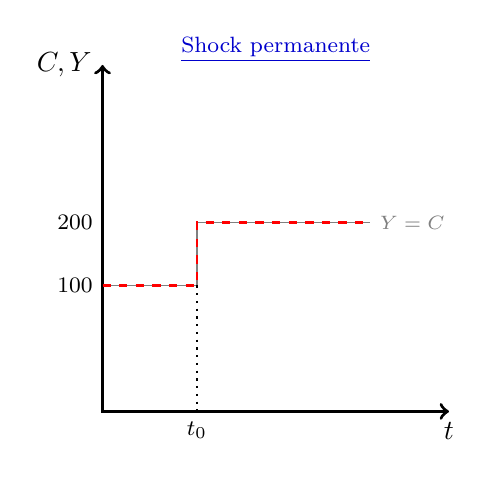
\begin{tikzpicture}[scale=0.4]
    \node[] at(5.5,11.5) {\footnotesize \textcolor{blue!80!black}{\underline{Shock permanente}}};
    \draw[very thick,<->] (0,11) node[left]{$C,Y$}--(0,0)--(11,0) node[below]{$t$};
    \draw[thin, gray](0, 4)--(3, 4)--(3,6)--(8.5,6) node[right] {\scriptsize $Y=C$};
    \draw[thick, dashed, red](0, 4)--(3, 4)--(3,6)--(8.5,6);
    \draw[thick, dotted](3,4)--(3,0) node [below] {\footnotesize $t_0$};
    \node [left] at (0,4) {\footnotesize $100$};
    \node [left] at (0,6) {\footnotesize $200$};
    \end{tikzpicture}
    \footnotesize Para mantener el consumo estable, pasa \\ a consumir siempre su nuevo nivel de \\ ingreso (200)
    \end{center}


    \column{0.5\textwidth}
    \begin{center}
    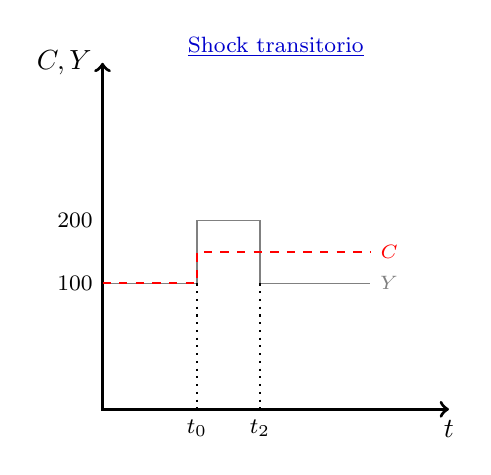
\begin{tikzpicture}[scale=0.4]
    \node[] at(5.5,11.5) {\footnotesize \textcolor{blue!80!black}{\underline{Shock transitorio}}};
    \draw[very thick,<->] (0,11) node[left]{$C,Y$}--(0,0)--(11,0) node[below]{$t$};
    \draw[thin, gray](0, 4)--(3, 4)--(3,6)--(5,6)--(5,4)--(8.5,4)node[right] {\scriptsize $Y$};
    \draw[thick, dashed, red](0, 4)--(3, 4)--(3,5)--(8.5,5) node[right] {\scriptsize $C$};
    \draw[thick, dotted](3,4)--(3,0) node [below] {\footnotesize $t_0$};
    \draw[thick, dotted](5,4)--(5,0) node [below] {\footnotesize $t_2$};
    \node [left] at (0,4) {\footnotesize $100$};
    \node [left] at (0,6) {\footnotesize $200$};
    \end{tikzpicture}
    \footnotesize Aumenta un poco su consumo y \\ ahorra el resto para sostener un nivel \\ de consumo más alto que el original.
    \end{center}

    
\end{columns}


\end{frame}


\begin{frame}{Shocks de ingreso futuro}
\small Una persona espera recibir un shock permanente de ingreso dentro de 6 periodos 
\begin{center}
\begin{figure}[H]
\begin{center}
\begin{tikzpicture}[scale=0.47]
\draw[very thick,<->] (0,11) node[left]{$C,Y$}--(0,0)--(11,0) node[below]{$t$};
\draw[thin, gray](0, 4)--(6, 4)--(6,6)--(8.5,6)node[right] {\scriptsize $Y$};
\draw[thick, dashed, red](0, 4)--(3, 4)--(3,5)--(8.5,5) node[right] {\scriptsize $C$};
\draw[thick, dotted](3,4)--(3,0) node [below] {\footnotesize $t_0$};
\draw[thick, dotted](6,4)--(6,0) node [below] {\footnotesize $t_0+6$};
%\draw[thick, dashed](0, 4)--(3,4)--(3,6)--(5,6);
\end{tikzpicture}
\end{center}
\end{figure}
\end{center}  
\vspace{-1mm}
\small La persona se endeudará hoy ($t_0$) para aumentar su consumo y pagará la deuda en el futuro con el ingreso adicional que espera a partir del shock.
\end{frame}


\begin{frame}{Modelo de elección entre consumo presente y futuro}
    \begin{itemize} \small
        \item En vez de elegir entre consumir pizza y cerveza, ahora hay que elegir cuánto consumir entre hoy ($t$) y mañana ($t+1$).
        \item Vamos a representar el consumo de hoy $c_t$ en el eje $x$ y el consumo de mañana $c_{t+1}$ en el eje $y$. 
        \item Tenemos una dotación de ingresos en cada período ($y_t$, $y_{t+1}$)
        \item Si el crédito no existe, la restricción intertemporal es solo el punto $A$
    \end{itemize}

\begin{center}
\begin{figure}[h!]
\begin{center}
\begin{tikzpicture}[scale=0.4]
\draw[very thick,<->] (0,11) node[left]{\footnotesize $c_{t+1}$}--(0,0)--(11,0) node[below]{\footnotesize $c_{t}$};
%\draw[thin] (0,7)--(8,0);
 \draw[thick,gray, dashed](3.5, 3.95)--(3.5, 0);
  \draw[thick,gray, dashed](3.5, 3.95)--(0, 3.95);
 \node[below] at (3.5,0) {\footnotesize $y_t=c_t$};
  \node[left] at (0,3.95) {\footnotesize $y_{t+1}=c_{t+1}$};
  \draw[fill] (3.5,3.95) circle [radius =0.11] node[right]{$A$} ;
\end{tikzpicture}
\end{center}
\end{figure}
\end{center}  
\end{frame}

\begin{frame}{La restricción intertemporal \textbf{con} crédito}
    Si hay crédito, podemos armar una restricción presupuestaria jugando con la tasa de interés. Pensemos en los puntos extremos: \\ \vspace{1mm}
   \textcolor{blue!70!black}{\textbf{Maximizar el consumo de hoy}} 
    \begin{itemize} \small
        \item Tenemos que consumir lo que tenemos hoy ($y_t$) y pedir prestado (a una tasa de interés $r$) lo máximo que podemos devolver mañana.
         \item ¿Cuánto podemos pedir prestado? Si pedimos prestado un monto $a$, mañana tenemos que devolver $a\cdot(1+r)$. Si vamos a usar todo nuestro ingreso de mañana $y_{t+1}$ para devolver el préstamo:
             \[y_{t+1} = a \cdot (1+r)\]
         Lo máximo que podemos pedir prestado es $\frac{y_{t+1}}{(1+r)}$
         \item El máximo consumo de hoy es entonces:
                      \[c_{t} = y_t +\frac{y_{t+1}}{(1+r)}\]
    \end{itemize}
\end{frame}

\begin{frame}{La restricción intertemporal \textbf{con} crédito}
\begin{center}
\begin{figure}[H]
\begin{center}
\begin{tikzpicture}[scale=0.6]
\draw[very thick,<->] (0,11) node[left]{$c_{t+1}$}--(0,0)--(11,0) node[below]{$c_{t}$};
%\draw[thin] (0,7)--(8,0);
\draw[thick,gray, dashed](3.5, 3.95)--(3.5, 0);
\draw[thick,gray, dashed](3.5, 3.95)--(0, 3.95);
\node[below] at (3.5,0) {\footnotesize $y_t$};
\node[left] at (0,3.95) {\footnotesize $y_{t+1}$};
\draw[fill] (3.5,3.95) circle [radius =0.11] ;
\draw[fill, blue] (8,0) circle [radius =0.11] ;
\node[below, blue] at (8,0) {\footnotesize $y_t + \frac{y_{t+1}}{(1+r)}$};
% \node[left] at (0,7) {\footnotesize $y_{t+1}+(1+r)y_t$};

\end{tikzpicture}
\end{center}
\end{figure}
\end{center} 
\end{frame}


\begin{frame}{La restricción intertemporal \textbf{con} crédito}
   \textcolor{blue!70!black}{\textbf{Maximizar el consumo de mañana}} 
    \begin{itemize} \small
        \item Esto implica no consumir nada hoy y ahorrar el 100\% del ingreso.
        \item Si ahorramos $y_t$ hoy, mañana nos devolverán $y_t \cdot(1+r)$
        \item ¿Cuánto es el máximo consumo de mañana? Nuestro ingreso $y_{t+1}$ más lo que ahorramos:
            \[c_{t+1} = y_{t+1} +y_{t}\cdot(1+r)\]
    \end{itemize}
\vspace{2mm}
   \textcolor{blue!70!black}{\textbf{La restricción intertempral}} \\
    La pendiente de la restricción presupuestaria (TMT) es $-(1+r)$
    \begin{itemize} \small
        \item La tasa de interés es el costo de oportunidad de consumir un peso hoy.
        \item Cuanto más alta sea $r$, más empinada será la restricción: 
            \begin{itemize}  \footnotesize
            \item Cada peso ahorrado hoy equivaldría a mayor plata para consumir mañana (mayor intersección con eje $y$)
            \item Menos plata que puedo tomar prestada hoy (menor intersección con eje $x$)
            \end{itemize}
    \end{itemize}
\end{frame}


\begin{frame}{La restricción intertemporal \textbf{con} crédito}
\begin{center}
\begin{figure}[H]
\begin{center}
\begin{tikzpicture}[scale=0.6]
\draw[very thick,<->] (0,11) node[left]{$c_{t+1}$}--(0,0)--(11,0) node[below]{$c_{t}$};
\draw[thick,gray, dashed](3.5, 3.95)--(3.5, 0);
\draw[thick,gray, dashed](3.5, 3.95)--(0, 3.95);
\node[below] at (3.5,0) {\footnotesize $y_t$};
\node[left] at (0,3.95) {\footnotesize $y_{t+1}$};
\draw[fill] (3.5,3.95) circle [radius =0.11] ;
\draw[fill] (8,0) circle [radius =0.11] ;
\node[below] at (8,0) {\footnotesize $y_t + \frac{y_{t+1}}{(1+r)}$};

\node[left, blue] at (0,7) {\footnotesize $y_{t+1}+(1+r)y_t$};
\draw[fill, blue] (0,7) circle [radius =0.11] ;

\only<2->{
\draw[semithick] (0,7)--(8,0);
\node[left] at (0,7) {\footnotesize $y_{t+1}+(1+r)y_t$};
\draw[fill] (0,7) circle [radius =0.11] ;
}
\end{tikzpicture}
\end{center}
\end{figure}
\end{center} 
\end{frame}


\begin{frame}{La curva de indiferencia}
Sabemos que las personas buscan suavizar su consumo.\\ \vspace{1mm}
El consumo en el tiempo tiene \textbf{utilidad marginal decreciente}: si consumo mucho hoy, cada unidad adicional que consuma hoy me da menos satisfacción que la anterior.
\begin{center}
\begin{figure}[H]
\begin{center}
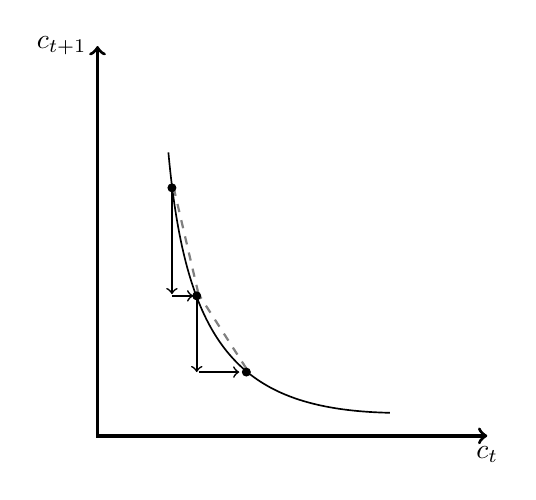
\begin{tikzpicture}[scale=0.45]
\draw[very thick,<->] (0,11) node[left]{$c_{t+1}$}--(0,0)--(11,0) node[below]{$c_{t}$};
%\draw[semithick] (2,8).. controls (2.5,2.5) and (4,1) ..(8,0);
\draw[semithick] (2,8).. controls (2.5,2.5) and (4,0.75) ..(8.25,0.65);
 \draw[thick,gray, dashed](2.15, 7)--(2.85, 4);
   \draw[fill] (2.1,7) circle [radius =0.11] ;
 \draw[thick,gray, dashed](4.2, 1.9)--(2.85, 4);      
      \draw[fill] (2.8,3.95) circle [radius =0.11] ;
\draw[fill] (4.2,1.8) circle [radius =0.11] ;      
\draw[semithick, ->] (2.1,7)--(2.1,4);
\draw[semithick, ->] (2.1,3.95)--(2.7,3.95);
\draw[semithick, ->] (2.8,3.95)--(2.8,1.8);
\draw[semithick, ->] (2.85,1.8)--(4,1.8);
\end{tikzpicture}
\end{center}
\end{figure}
\end{center}  
\end{frame}

\begin{frame}{El equilibrio}
\small Asumiendo que $y_t<y_{t+1}$, para maximizar la utilidad deberíamos tomar prestado algo para consumir hoy un poco más de lo que nos permite nuestro ingreso

\begin{center}
\begin{figure}[H]
\begin{center}
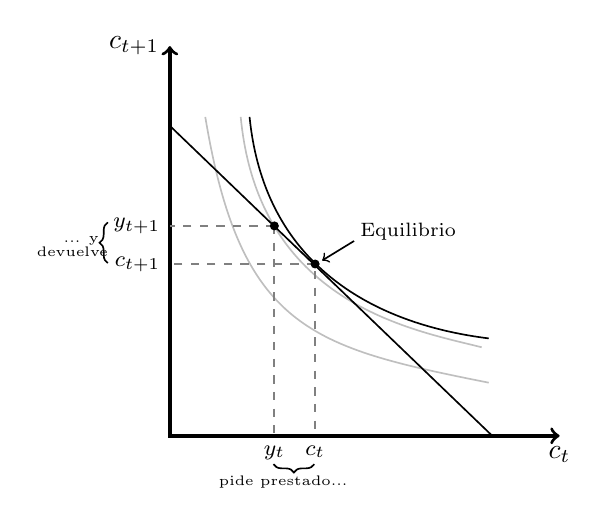
\begin{tikzpicture}[scale=0.45]
\draw[very thick,<->] (0,11) node[left]{$c_{t+1}$}--(0,0)--(11,0) node[below]{$c_{t}$};
\draw[semithick, gray!50] (1,9).. controls (2,3) and (4, 2.5) .. (9, 1.5) ;
\draw[semithick, gray!50] (2,9).. controls (2.5,3.75) and (6.8, 3) .. (8.8, 2.5);
\draw[semithick] (2.25,9).. controls (2.75,4) and (7, 3) .. (9, 2.75);
\draw[semithick] (0,8.75)--(9.1,0);
 \draw[thick,gray, dashed](4.1, 4.65)--(4.1, 0);
 \draw[thick,gray, dashed](4.1, 4.85)--(0, 4.85);
 \draw[fill] (4.1,4.85) circle [radius =0.11] ;  
 \node[below] at (4.1,0) {\footnotesize $c_t$};
 \node[left] at (0,4.85){\footnotesize $c_{t+1}$};
 \draw[thick,gray, dashed](2.95, 5.925)--(2.95, 0);
 \draw[thick,gray, dashed](2.95, 5.925)--(0, 5.925);
 \draw[fill] (2.95,5.925) circle [radius =0.11] ;   
 \node[below] at (2.95,0) {\footnotesize $y_t$};
 \node[left] at (0,5.925){\footnotesize $y_{t+1}$};
 \node [right] at (5.1,5.75) {\scriptsize  Equilibrio}  ;
\draw[semithick, <-] (4.3,4.95)--(5.2,5.5);
\draw [semithick,decorate,decoration={brace,amplitude=3pt,mirror},xshift=5pt,yshift=0pt](2.75,-0.8) -- (3.9,-0.8);
\draw (3.2,-1.3) node[]{\tiny pide prestado...};
\draw [semithick,decorate,decoration={brace,amplitude=3pt,mirror},xshift=0pt,yshift=5pt](-1.75,5.85) -- (-1.75,4.7);
\draw (-2.5,5.5) node[]{\tiny ... y};
\draw (-2.75,5.2) node[]{\tiny devuelve};
\end{tikzpicture}
\end{center}
\end{figure}
\end{center}  
\small En el equilibrio, el consumidor iguala la TMS entre el consumo de hoy y mañana a la tasa de interés de mercado (TMT).
\end{frame}


\begin{frame}{El efecto de un cambio en la tasa de interés}
    \begin{itemize}
        \item La tasa de interés no es otra cosa que el precio del consumo presente relativo al consumo futuro, entonces el cambio en la tasa de interés se puede descomponer en un efecto ingreso y un efecto sustitución.
        \begin{itemize}
            \item \textbf{ES}: lleva a consumir menos (ahorrar más) ante aumentos en la tasa de interés. Se vuelve más atractivo ahorrar porque aumenta el costo de oportunidad de consumir en el presente.
            \item \textbf{EI}: que me vuelva más rico o no depende de mi situación inicial:
            \begin{itemize}
                \item Si soy un ahorrista neto, me vuelvo más rico porque el valor presente de mis ahorros aumenta.
                \item Si soy un deudor neto, me vuelvo más pobre porque el valor presente de mis deudas aumenta.
            \end{itemize}
            \item En general, el efecto sustitución es más fuerte que el efecto ingreso porque el efecto ingreso se compensa entre deudores y acreedores.
        \end{itemize}
        \item Por eso, ante aumentos en la tasa de interes estos modelos muestran que aumenta el ahorro (baja el consumo) y visceversa ante caidas en la tasa de interes.
    \end{itemize}
\end{frame}



\begin{frame}{El efecto de un cambio en la tasa de interés}
\small Si la tasa de interés aumenta, la restricción pivotea. Dado que $ES >EI$, el nuevo equilibrio implica que pedimos menos prestado (es más costoso devolver el préstamo)

\begin{center}
\begin{figure}[H]
\begin{center}
\begin{tikzpicture}[scale=0.5]
\draw[very thick,<->] (0,11) node[left]{$c_{t+1}$}--(0,0)--(11,0) node[below]{$c_{t}$};
%\draw[semithick, gray!50] (1,9).. controls (2,3) and (4, 2.5) .. (9, 1.5) ;
\draw[semithick, blue] (2,9).. controls (2.5,3.75) and (6.8, 3) .. (8.8, 2.5);
\draw[semithick, gray!50] (2.25,9).. controls (2.75,4) and (7, 3) .. (9, 2.75);
\draw[semithick, gray!50] (0,8.75)--(9.1,0);
\draw[semithick, blue] (0,9.75)--(7.25,0);
 \draw[thin,gray!50, dashed](4.1, 4.65)--(4.1, 0);
 \draw[thin,gray!50, dashed](4.1, 4.85)--(0, 4.85);
 \draw[fill, gray] (4.1,4.85) circle [radius =0.11];  
 \node[below, gray!50] at (4.1,0) {\tiny $c_t$};
 \node[left, gray!50] at (0,4.85){\tiny $c_{t+1}$};

  \draw[fill, blue] (3.35,5.25) circle [radius =0.11];  
 \node[below, blue!70] at (3.5,0) {\tiny $c_t$};
 \node[left, blue!70] at (0,5.4){\tiny $c_{t+1}$};
 \draw[thin,blue!70, dashed](3.35,5.25)--(3.35, 0);
 \draw[thin,blue!70, dashed](3.35,5.25)--(0, 5.25);
  
 \draw[thin,gray, dashed](2.95, 5.925)--(2.95, 0);
 \draw[thin,gray, dashed](2.95, 5.925)--(0, 5.925);
 \draw[fill] (2.95,5.925) circle [radius =0.11] ;   
 \node[below] at (2.95,0) {\tiny $y_t$};
 \node[left] at (0,5.925){\tiny $y_{t+1}$};
% \node [right] at (5.1,5.75) {\scriptsize  Equilibrio}  ;
%\draw[semithick, <-] (4.3,4.95)--(5.2,5.5);
\draw [semithick, blue, decorate,decoration={brace,amplitude=3pt,mirror, blue},xshift=5pt,yshift=0pt](2.75,-0.8) -- (3.5,-0.8);
\draw (3.2,-1.3) node[blue]{\tiny pide prestado...};
\draw [semithick,blue , decorate,decoration={brace,amplitude=3pt,mirror},xshift=0pt,yshift=5pt](-1.75,5.85) -- (-1.75,5.2);
\draw (-2.65,5.7) node[blue]{\tiny ... y};
\draw (-2.85,5.4) node[blue]{\tiny devuelve};
\end{tikzpicture}
\end{center}
\end{figure}
\end{center}  
\end{frame}


\begin{frame}{El efecto de un cambio en la tasa de interés}
\small Pensemos un caso donde ahorremos: asumimos que solo tenemos ingresos hoy y no mañana ($y_{t+1}=0$). Si aumenta la tasa de interés, la restricción pivotea sobre $y_{t}$. El resultado es consumir menos hoy (tenemos mayores incentivos a ahorrar).

\begin{center}
\begin{figure}[h!]
\begin{center}
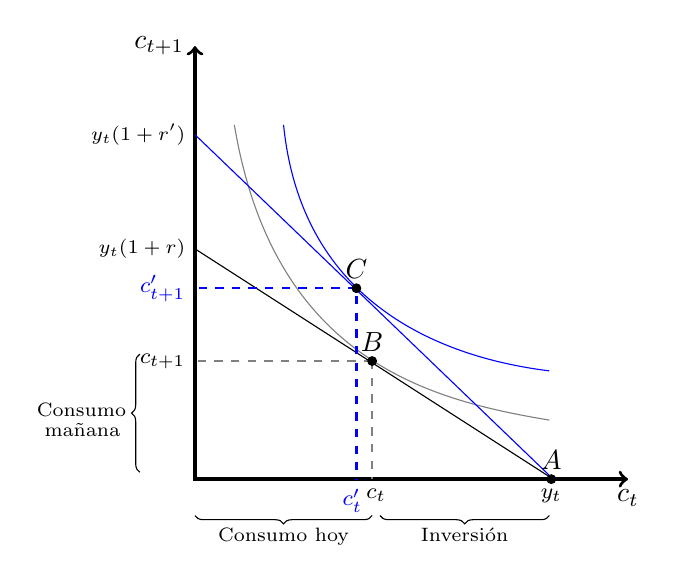
\begin{tikzpicture}[scale=0.5]
\draw[very thick,<->] (0,11) node[left]{$c_{t+1}$}--(0,0)--(11,0) node[below]{$c_{t}$};
\draw[thin, gray] (1,9).. controls (2,3) and (6, 2) .. (9, 1.5) ;
%\draw[thin, gray] (0.25,9).. controls (0.5,3) and (7, 1) .. (9, 0);
\draw[thin, blue] (2.25,9).. controls (2.75,4) and (7, 3) .. (9, 2.75);
\draw[thin, blue] (0,8.75)--(9.1,0);
\draw[thin] (0,5.85)--(9.1,0);
  \draw[thick,blue, dashed](4.1, 4.65)--(4.1, 0);
  \draw[thick,blue, dashed](4.1, 4.85)--(0, 4.85);
  \draw[fill] (4.1,4.85) circle [radius =0.11] node[above] {$C$};  
  \node[below, blue] at (4,0) {\footnotesize $c'_t$};
  \node[left, blue] at (0,4.85){\footnotesize $c'_{t+1}$};
%  \draw[thick,gray, dashed](2.95, 5.925)--(2.95, 0);
%  \draw[thick,gray, dashed](2.95, 5.925)--(0, 5.925);
  \draw[thick,gray, dashed](4.5, 3)--(4.5, 0);
  \draw[thick,gray, dashed](4.5, 3)--(0, 3) ; 
  \node[below] at (4.6,0) {\footnotesize $c_t$};
  \node[left] at (0,3){\footnotesize $c_{t+1}$};
  \draw[fill] (4.5,3) circle [radius =0.11] node[above] {$B$};   
    \draw[fill] (9.05,0) circle [radius =0.11] node [below] {\footnotesize $y_t$} node[above] {$A$};   
  \node[left] at (0,5.85){\scriptsize $ y_t (1+r)$};   
  \node[left] at (0,8.75){\scriptsize $ y_t (1+r')$};
   \draw [thin,decorate,decoration={brace,amplitude=3pt},xshift=0pt,yshift=5pt](-1.4,0) -- (-1.4,3);  
  \draw [thin,decorate,decoration={brace,amplitude=3pt, mirror},xshift=0pt,yshift=5pt](0,-1.1) -- (4.5,-1.1); 
  
    \draw [thin,decorate,decoration={brace,amplitude=3pt, mirror},xshift=0pt,yshift=5pt](4.7,-1.1) -- (9,-1.1); 
  \node[left] at (-1.5,1.75){\scriptsize Consumo};   
    \node[left] at (-1.65,1.25){\scriptsize mañana};
  \node[below] at (2.25,-1){\scriptsize Consumo hoy};      
    \node[below] at (6.85,-1){\scriptsize Inversión};     
\end{tikzpicture}
\end{center}
\end{figure}
\end{center}  
\end{frame}

\begin{comment}
\begin{frame}{Apalancamiento}
   \begin{center}
\begin{figure}[H]
\renewcommand{\figurename}{Figure}
\begin{center}
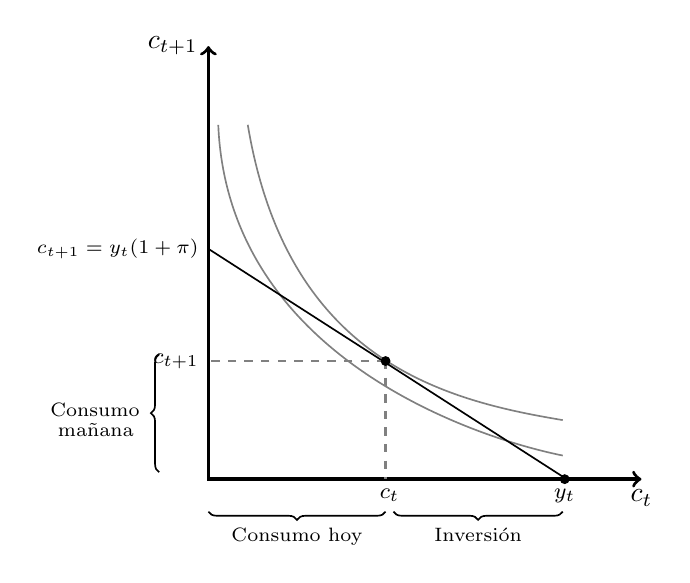
\begin{tikzpicture}[scale=0.5]
\draw[very thick,<->] (0,11) node[left]{$c_{t+1}$}--(0,0)--(11,0) node[below]{$c_{t}$};
\draw[semithick, gray] (1,9).. controls (2,3) and (6, 2) .. (9, 1.5) ;
%\draw[semithick, gray] (0.25,9).. controls (0.5,3) and (7, 1) .. (9, 0);
\draw[semithick, gray] (0.25,9).. controls (0.5,3) and (7, 1) .. (9, 0.6);
\draw[semithick] (0,5.85)--(9.1,0);
  \draw[thick,gray, dashed](4.5, 3)--(4.5, 0);
  \draw[thick,gray, dashed](4.5, 3)--(0, 3);
  \node[below] at (4.6,0) {\footnotesize $c_t$};
  \node[left] at (0,3){\footnotesize $c_{t+1}$};
  \draw[fill] (4.5,3) circle [radius =0.11] ;   
    \draw[fill] (9.05,0) circle [radius =0.11] node [below] {\footnotesize $y_t$} ;   
  \node[left] at (0,5.85){\scriptsize $c_{t+1} = y_t (1+\pi)$};   
 \draw [semithick,decorate,decoration={brace,amplitude=3pt},xshift=0pt,yshift=5pt](-1.25,0) -- (-1.25,3);  
  \draw [semithick,decorate,decoration={brace,amplitude=3pt, mirror},xshift=0pt,yshift=5pt](0,-1) -- (4.5,-1); 
  
    \draw [semithick,decorate,decoration={brace,amplitude=3pt, mirror},xshift=0pt,yshift=5pt](4.7,-1) -- (9,-1); 
  \node[left] at (-1.5,1.75){\scriptsize Consumo};   
    \node[left] at (-1.65,1.25){\scriptsize mañana};
  \node[below] at (2.25,-1){\scriptsize Consumo hoy};      
    \node[below] at (6.85,-1){\scriptsize Inversión};     
\end{tikzpicture}
\end{center}
\end{figure}
\end{center}   
\end{frame}


\begin{frame}{Apalancamiento}
    \begin{center}
\begin{figure}[H]
\renewcommand{\figurename}{Figure}
\begin{center}
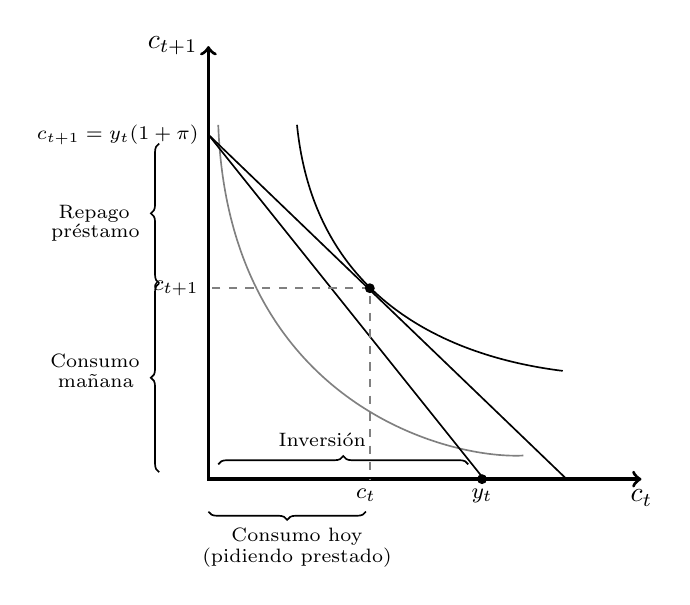
\begin{tikzpicture}[scale=0.5]
\draw[very thick,<->] (0,11) node[left]{$c_{t+1}$}--(0,0)--(11,0) node[below]{$c_{t}$};
%\draw[semithick, gray] (0.25,9).. controls (0.5,2) and (6, 0.5) .. (7, 0);
\draw[semithick, gray] (0.25,9).. controls (0.5,2) and (6, 0.5) .. (8, 0.6);
\draw[semithick] (2.25,9).. controls (2.75,4) and (7, 3) .. (9, 2.75);
\draw[semithick] (0,8.75)--(9.1,0);
\draw[semithick] (0,8.75)--(7,0);
  \draw[thick,gray, dashed](4.1, 4.65)--(4.1, 0);
  \draw[thick,gray, dashed](4.1, 4.85)--(0, 4.85);
  \draw[fill] (4.1,4.85) circle [radius =0.11] ;  
  \node[below] at (4,0) {\footnotesize $c_t$};
  \node[left] at (0,4.85){\footnotesize $c_{t+1}$};
    \draw[fill] (6.95,0) circle [radius =0.11] node [below] {\footnotesize $y_t$} ;   
  \node[left] at (0,8.75){\scriptsize $c_{t+1} = y_t (1+\pi)$}; 
   \draw [semithick,decorate,decoration={brace,amplitude=3pt},xshift=0pt,yshift=5pt](-1.25,0) -- (-1.25,4.8); 
      \draw [semithick,decorate,decoration={brace,amplitude=3pt,mirror},xshift=0pt,yshift=5pt](-1.25,8.35) -- (-1.25,4.8); 
  \draw [semithick,decorate,decoration={brace,amplitude=3pt, mirror},xshift=0pt,yshift=5pt](0,-1) -- (4,-1); 
\draw [semithick,decorate,decoration={brace,amplitude=3pt},xshift=0pt,yshift=5pt](0.25,0.2) -- (6.6,0.2); 
  \node[left] at (-1.5,3){\scriptsize Consumo};   
    \node[left] at (-1.65,2.5){\scriptsize mañana};
  \node[below] at (2.25,-1){\scriptsize Consumo hoy};
  \node[below] at (2.25,-1.5){\scriptsize (pidiendo prestado)};
    \node[left] at (4.25,1){\scriptsize Inversión};
      \node[left] at (-1.75,6.75){\scriptsize Repago };   
    \node[left] at (-1.5,6.25){\scriptsize préstamo};
\end{tikzpicture}
\end{center}
\end{figure}
\end{center} 
\end{frame}


\begin{frame}{El Gran Elon}
   \begin{figure} [H]
    \centering
    \href{https://twitter.com/Stelladmarco/status/1103059259586052097}{
    
\includegraphics[scale=0.5]{Slides Principios de Economia/Figures/C31.9.png}}
\end{figure} 
\end{frame} 

\end{comment}

\begin{frame}{Apalancamiento}
   \begin{itemize}
       \item ¿Qué sucede si al préstamo que pedimos lo usamos para invertir?
       \item Al uso de deuda para financiar un proyecto lo denominaremos \textbf{apalancamiento}.
       \item ¿Cuándo conviene "apalancarse"? La regla básica de decisión implica comparar el retorno del proyecto de inversión ($\pi$) con costo de financiarlo ($r$).
          \begin{itemize}
       \item \textcolor{blue!70!black}{Siempre que la tasa de retorno sea mayor a la tasa de interés ($\pi>r$), conviene pedir prestado para invertir.} 
          \end{itemize} 
       \item Ejemplo: pedimos prestado $\$1000$ a una tasa de interés $r=10\%$ y lo invertimos en un proyecto que promete un retorno de $\pi=20\%$.
          \begin{itemize}
        \item Tenemos que devolver $1000\times(1+10\%)=1100$, pero con el proyecto ganamos $1000\times(1+20\%)=1200\rightarrow$ ganancia neta $=100$  
       \item ¿Y si $\pi=8\%$? Ahora con el proyecto ganamos $1080$, que es menor al costo de financiarlo. Nos endeudamos para perder plata!
          \end{itemize} 
   \end{itemize} 
\end{frame}


\begin{frame}{Otras teorías del ahorro}
   \begin{itemize}
       \item Ciclo de vida
       \item Hipotecas revertidas
       \item Los tests de Shea
       \item Ahorro precautorio
       \item La fuerza de los defaults
       \item Present bias
       \item Ubank
   \end{itemize} 
\end{frame}


\begin{frame}{La inversión: valor presente}
    La inversión se decide en base al valor presente de los flujos futuros de ingreso que genera un determinado proyecto.
    \begin{equation}
        VPN = I_0 + \sum_{t=1} ^{T} \frac{1}{(1+r)^t} R_t,
    \end{equation}
    \begin{itemize}
        \item $r$ es el costo del capital.
        \item $I_0$ es el costo inicial.
        \item ¿Cuanta plata necesito hoy para tener $R_t$ en el futuro? Como entre ahora y $t$, cualquier dinero podemos ponerlo a rendir un interés del mercado, el equivalente hoy de un dinero futuro será menor.
        \item Si el VPN$>0$, entonces convendría invertir.
        \item Si VPN $<0$ no convendría.
        \item ¿Tarjetas de crédito? ¿Inflación?
    \end{itemize}
\end{frame}




\begin{frame}{Demanda agregada y el mercado de crédito}

$$ Y = C(r) + I(r) + G $$

\centering \small{donde r es la tasa de interés real}

\begin{itemize}
\item En una economía cerrada:
\[
\underbrace{Y - C(r) - G}_{\text{Ahorro}} = \underbrace{I(r)}_{\text{Inversión}} 
\]
\end{itemize}
\begin{itemize}
\item El ahorro es la oferta en el mercado de crédito y la inversión es el demandante de ese crédito
\item Los ahorros son intermediados por el sector financiero hacia inversiones reales.
\item Economías que ahorran mucho invierten mucho (China, Japón), economías que ahorran poco invierten menos (Brasil, Argentina)! 
\end{itemize}
\end{frame}


\begin{frame}{El mercado de crédito}
\begin{center}
\begin{figure}[H]
\renewcommand{\figurename}{Figure}
\begin{center}
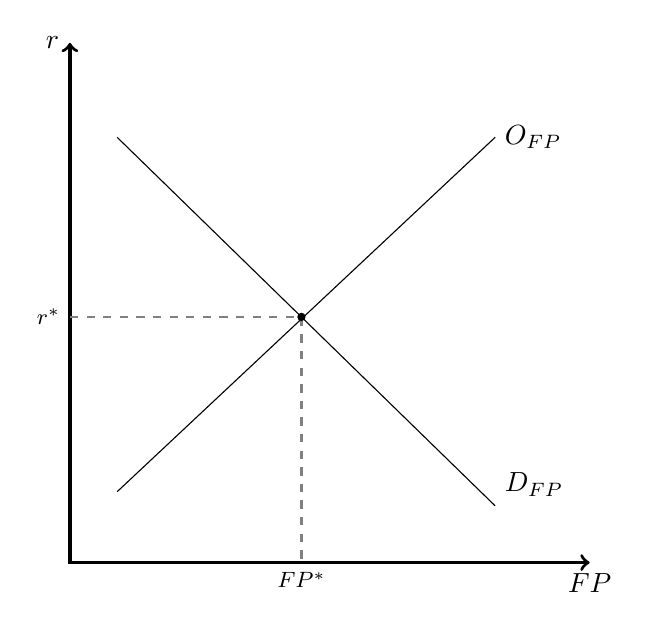
\begin{tikzpicture}[scale=0.6]
\draw[very thick,<->] (0,11) node[left]{$r$}--(0,0)--(11,0) node[below]{$FP$};

%\node[] at(5,-1.5) {\underline{Mercado de Crédito}};
\draw[thin](1,1.5)--(9,9) node [right] {$O_{FP}$};
\draw[thin](1,9)--(9,1.2) node [above right] {$D_{FP}$};
\draw[thick,dashed,gray] (0,5.2)--(4.9,5.2)--(4.9,0);
\draw[fill] (4.9,5.2) circle [radius =0.075]; 
\node[below] at (4.9,0) {\footnotesize $FP^{*}$};
\node[left] at (0,5.2) {\footnotesize $r^{*}$};
\end{tikzpicture}
\end{center}
\end{figure}
\end{center}  
\end{frame}

\begin{frame}{El mercado de crédito}
    \begin{itemize}
        \item La tasa de interés de equilibrio se alcanza cuando la demanda de crédito (demanda de fondos prestables) se iguala con la oferta de crédito (oferta de fondos prestables).
        \item Un aumento en la inversión desplaza la curva de crédito hacia arriba (se demandan más prestamos), lo que aumenta la tasa de interés.
        \item En el mismo sentido:
        \begin{itemize}
            \item Un aumento en la deuda del gobierno (financia déficit con deuda).
        \end{itemize}
        \item Como en estos dos éltimos casos aumenta la tasa de interés, eso hará caer la inversión (en equilibrio), que es lo que llamamos \textit{crowding out}.
        \item Un aumento en el ahorro desplaza la curva de oferta de fondos prestables hacia abajo, permitiendo una menor tasa de interés de equilibrio.
    \end{itemize}
    
\end{frame}

\begin{frame}{El mercado de crédito}
    \begin{center}
\begin{figure}[H]
\renewcommand{\figurename}{Figure}
\begin{center}
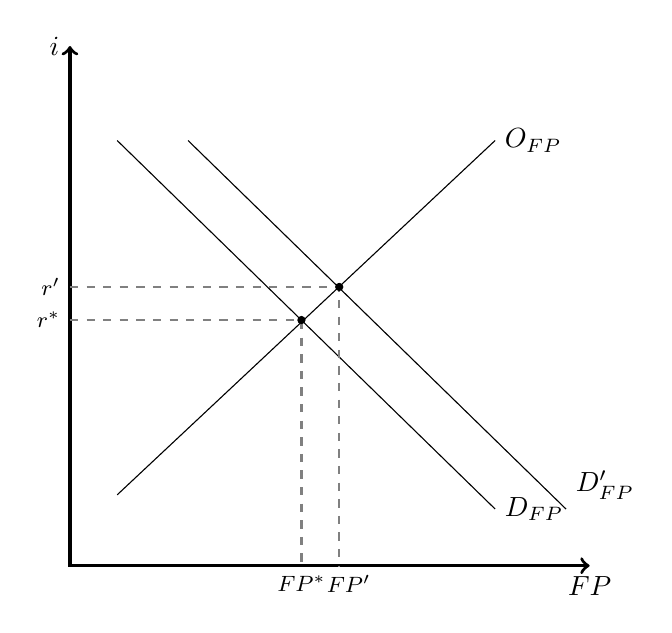
\begin{tikzpicture}[scale=0.6]
\draw[very thick,<->] (0,11) node[left]{$i$}--(0,0)--(11,0) node[below]{$FP$};
\draw[thin](1,1.5)--(9,9) node [right] {$O_{FP}$};
\draw[thin](1,9)--(9,1.2) node [right] {$D_{FP}$};
\draw[thin](2.5,9)--(10.5,1.2) node [above right] {$D_{FP}'$};
\draw[thick,dashed,gray] (0,5.2)--(4.9,5.2)--(4.9,0);
\draw[thick,dashed,gray] (0,5.9)--(5.7,5.9)--(5.7,0);
\draw[fill] (4.9,5.2) circle [radius =0.075]; 
\draw[fill] (5.7,5.9) circle [radius =0.075]; 
\node[below] at (4.9,0) {\footnotesize $FP^{*}$};
\node[left] at (0,5.2) {\footnotesize $r^{*}$};
\node[below] at (5.9,0) {\footnotesize $FP'$};
\node[left] at (0,5.9) {\footnotesize $r'$};
\end{tikzpicture}
\end{center}
\end{figure}
\end{center}  
\end{frame}



\end{document}